\chapter{Appendix}
%
\begin{figure}[!ht]%
    \centering
    %\subfloat[Amplitude \(\hat{U}\)\label{subfig:fig1pulsAmplitude}]{\includegraphics[width=0.45\textwidth]{messdaten/Fig.1_pulsAmplitude.jpg}}%
    \hspace{.05\textwidth}
    %\subfloat[Fall Time \(t_{f}\)\label{subfig:fig2fallTime}]{\includegraphics[width=0.45\textwidth]{messdaten/Fig.2_fallTime.jpg}}%
    \hspace{.2\textwidth}
   % \subfloat[Rise Time \(t_{r}\)\label{subfig:fig3riseTime}]{\includegraphics[width=0.45\textwidth]{messdaten/Fig.3_riseTime.jpg}}%
    \hspace{.05\textwidth}
    %\subfloat[Pulse Width \(t_p\)\label{subfig:fig4pulseWidth}]{\includegraphics[width=0.45\textwidth]{messdaten/Fig.4_pulseWidth.jpg}}%
    \hspace{.2\textwidth}
    %\subfloat[Recovery Time \(t_{r}\)\label{subfig:fig5recoveryTime}]{\includegraphics[width=0.45\textwidth]{messdaten/Fig.5_recoveryTime.jpg}}%
    \caption[Oszillograms]{During the course of the experiment captured oscillograms.}%
    \label{fig:oscillograms}
\end{figure}
%
\newpage
%
\begin{table}[!ht]%
    \centering
    \caption[Handwritten notes]{Handwritten notes corresponding each measurement.}%
    %\subfloat[GMT characteristics.\label{subfig:3-1}]{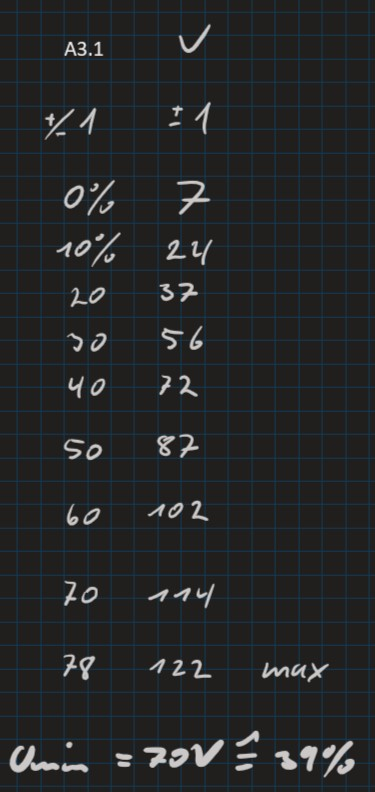
\includegraphics[height=0.7\textheight]{messdaten/handschriftliches/3-1.jpg}}
    \hspace{2mm}
    %\subfloat[Absorption characteristics of materials.\label{subfig:3-3}]{\includegraphics[height=0.7\textheight]{messdaten/handschriftliches/3-3.jpg}}
\end{table}
\begin{table}[!ht]%
    \ContinuedFloat
    \caption[Handwritten notes]{Handwritten notes corresponding each measurement.}%
    %\subfloat[Angular dependency of the count rate.\label{subfig:3-2}]{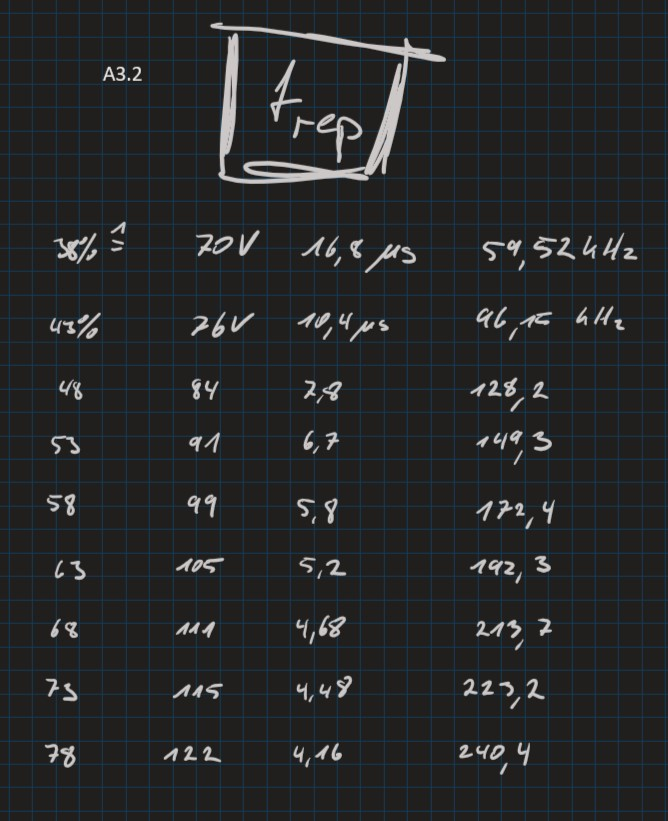
\includegraphics[width=0.45\textwidth]{messdaten/handschriftliches/3-2.jpg}}%
    \hspace{2mm}%
    %\subfloat[Absorption characteristics of materials.\label{subfig:3-4}]{\includegraphics[width=0.45\textwidth]{messdaten/handschriftliches/3-4.jpg}}%
\end{table}
\begin{table}[!ht]%
    \ContinuedFloat
    \caption[Handwritten notes]{Handwritten notes corresponding each measurement.}%
    %\subfloat[Background radiation.\label{subfig:3-5}]{\includegraphics[width=0.45\textwidth]{messdaten/handschriftliches/3-5.jpg}}
    \hspace{2mm}%
    %\subfloat[Natural radiation.\label{subfig:3-6}]{\includegraphics[width=0.45\textwidth]{messdaten/handschriftliches/3-6.jpg}}
\end{table}